\documentclass[aspectratio=169]{beamer}
\usepackage[utf8]{inputenc}
\usepackage{hyperref}
\usepackage{amsmath,amsfonts,amsthm,bm}
\usepackage{color}
\usepackage{minted}
\usepackage{graphicx} % Allows including images
\usepackage{booktabs} % Allows the use of \toprule, \midrule and \bottomrule in tables
\usepackage{tikz}
\usepackage[version=3]{mhchem}
\usepackage{pgfplots}
\pgfplotsset{compat=1.16} 
\setminted{fontsize=\scriptsize}

\hypersetup{
    colorlinks=true,
    linkcolor=red,
    filecolor=magenta,      
    urlcolor=red,
}

\DeclareMathOperator*{\argmax}{argmax}
\DeclareMathOperator*{\argmin}{argmin}
\let \vec \mathbf

\newcommand{\classname}{NANOx81R}

\mode<presentation> {
    \usetheme{CambridgeUS}
    \setbeamertemplate{footline}[text line]{%
      \parbox{\linewidth}{\vspace*{-8pt}\classname\hfill\insertpagenumber}}

    %\setbeamertemplate{footline}[page number]
    \setbeamertemplate{navigation symbols}{}
}


\title[Unsupervised Learning]{Unsupervised Learning}

\author{Shyue Ping Ong}
\institute[UCSD]{Aiiso Yufeng Li Family Department of Chemical and Nano Engineering\\
University of California, San Diego\\\url{http://materialsvirtuallab.org}}
\date{}

\begin{document}


\begin{frame}
    \titlepage % Print the title page as the first slide
\end{frame}


\begin{frame}{Overview}
    \tableofcontents
\end{frame}


\section{Preliminaries}

\begin{frame}{Preliminaries}
    \begin{itemize}
        \item Here, we will take a digression from the \textbf{supervised learning} that we have focused on so far, and go into \textbf{unsupervised learning}.
        \item In supervised learning, model development is carried out with a set of input/output examples (training data). 
        \item In unsupervised learning, the goal is to infer the properties of a set of data (e.g., its distribution) without training examples.
        \item We will include dimensionality reduction techniques within the umbrella of unsupervised learning.
    \end{itemize}
\end{frame}

\begin{frame}
\frametitle{Supervised vs Unsupervised Learning}
\begin{columns}
\column{0.5\textwidth}
Supervised learning
\begin{itemize}
    \item Learn from example inputs and outputs (labels).
    \item Clear metrics of success (e.g., maximum likelihood, MSE, MAE, etc.)
    \item Computationally efficient.
\end{itemize}
\column{0.5\textwidth}
Unsupervised Learning
\begin{itemize}
    \item Learn only from inputs.
    \item No rigorously-defined metric of success.
    \item Computationally complex.
\end{itemize}

\end{columns}
\end{frame} 


\section{Principal Component Analysis}


\begin{frame}{Principal Component Analysis (PCA)}
    \begin{itemize}
        \item Briefly alluded to in lecture on Linear Methods (regressing on derived input directions).
        \item Consider a dataset that has dimension $p$. The principal components provide a sequence of best linear approximations to that data, of all ranks $q \leq p$.
        \item Let the observations be $\vec{x_1}, \vec{x_2}, ..., \vec{x_N}$. The rank $q$ linear model for representing this data is given by:
        \begin{equation*}
            f(\vec{\lambda}) = \vec{\mu} + \vec{V_q}\vec{\lambda}
        \end{equation*}
        \item $\vec{\mu}$ is a location vector, $\vec{V_q}$ is a $p \times q$ matrix with $q$ orthogonal vectors, $\lambda$ is a length $q$ vector of parameters.
        \item We want to minimize the ``reconstruction error'',
        \begin{equation*}
            \min_{\vec{\mu}, \vec{V_q}, \vec{\lambda}} \sum_{i=1}^N ||\vec{x_i} - \vec{\mu} - \vec{V_q}\vec{\lambda_i}||^2
        \end{equation*}
    \end{itemize}
\end{frame} 

\begin{frame}{Solution}
    \begin{itemize}
        \item Minimizing wrt to $\vec{\mu}$ and $\vec{\lambda_i}$ gives
        \begin{eqnarray*}
        \hat{\vec{\mu}} & = & \bar{\vec{x}}\\
        \vec{\lambda_i} & = & \vec{V_q}^T(\vec{x_i}-\bar{\vec{x}})\\
    \end{eqnarray*}
        \item Need to solve:
        \begin{equation*}
          \min_{\vec{V_q}} \sum_{i=1}^N ||(\vec{x_i}-\bar{\vec{x}}) - \vec{V_q}\vec{V_q}^T(\vec{x_i}-\bar{\vec{x}})||^2
        \end{equation*}
    \end{itemize}
\end{frame} 

\begin{frame}{Solution, contd.}
    \begin{itemize}
        \item Construct singular value decomposition (SVD) of $\vec{X}$, the $N \times p$ matrix of centered $\vec{x_i}$.
        \begin{equation*}
            \vec{X} = \vec{U}\vec{D}\vec{V}^T
        \end{equation*}
        \item $\vec{U}$ is an $N \times p$ orthogonal matrix, $\vec{D}$ is a $p\times p $ diagonal matrix with singular values $d_1 > d_2 > ... > d_p$ and $\vec{V}$ is $p \times p$ orthogonal matrix with right singular vectors $\vec{v_1}, \vec{v_2}, ...\vec{v_p}$ as columns.
        \item $\vec{UD}$ are the principal components. 
        \item $\vec{Xv_1}$ has highest variance among all linear combination of features, followed by $\vec{Xv_2}$, $\vec{Xv_3}$, etc.
    \end{itemize}
\end{frame} 


\begin{frame}{Linear regression of bulk modulus on first two PCAs of elemental features}
\begin{figure}
    \centering
    \includegraphics[width=0.47\textwidth]{figures/pca-elements.png}
    \includegraphics[width=0.45\textwidth]{figures/pca-regression.png}
\end{figure}
\end{frame} 


\begin{frame}[fragile]{Code}
\inputminted{python}{example_sklearn_pca.py}
\end{frame} 


\begin{frame}{Example of linear regression on PCA components}
\begin{figure}
    \centering
    \includegraphics[width=0.45\textwidth]{figures/pca-regression.png}
\end{figure}
\end{frame} 

\begin{frame}{Extensions to PCA}
    \begin{itemize}
        \item Principal curves: smooth 1D curved approximation to data.
        \item Principal surfaces: curved 2D manifold approximation to data.
    \end{itemize}
\end{frame}

\section{Cluster Analysis}

\begin{frame}{Cluster Analysis}
    \begin{itemize}
        \item Cluster observations into groups so that pairwise differences within cluster tend to be smaller than differences between clusters.
        \begin{description}
        \item[Combinatorial algorithms] Model observed data with no underlying probability model.
        \item[Mixture modeling] Assumes samples are i.i.d. from some population with a probability density function.
        \item[Mode seekers] Estimate modes from PDF.
        \end{description}
    \end{itemize}
\end{frame}

\begin{frame}{K-means}
    \begin{itemize}
        \item One of the most popular iterative descent clustering methods.
        \item Often used with the Euclidean distance as the dissimlarity measure.
        \begin{equation*}
            d(x_i, x_i') = ||x_i - x_i'||^2
        \end{equation*}
        \item Classic k-means measure distance to centroids of clusters.
        \item Other distance metrics are possible: weighted Euclidean, periodic boundary condition distance, etc.
        \item Variants:
        \begin{itemize}
            \item $K$-medoids: Use one of points as cluster center instead of centroid. Removes influence of large outliers that produce large distances.
        \end{itemize}
    \end{itemize}
\end{frame}


\begin{frame}{K-means Algorithm}
    \begin{enumerate}
            \item Initialize a set of $k$ means (centroids), e.g., choosing $k$ observations to be the initial means (Forgy algo) or randomly assigns a cluster to each observation (random partition).
            \item Assign each observation to the cluster with the smallest distance, i.e., partition the observations using the Voronoi diagram generated by means.
            \item Recalculate the new means of the observations in the new clusters.
            \item Algorithm is converged when assignment no longer changes.
        \end{enumerate}
        \begin{figure}
            \includegraphics[width=0.18\textwidth]{figures/k-means-step-1.png}
            \includegraphics[width=0.18\textwidth]{figures/k-means-step-2.png}
            \includegraphics[width=0.18\textwidth]{figures/k-means-step-3.png}
            \includegraphics[width=0.18\textwidth]{figures/k-means-step-4.png}
            \caption{Four steps of K-means algorithm. Source: Wikipedia}
        \end{figure}
\end{frame} 


\begin{frame}{Practical considerations}
    \begin{itemize}
        \item K-means is often used for vector quantization, i.e., split a set of values into k levels.
        \item Determining $K$. Sometimes $K$ is based on goals, e.g., if you have a scientific / practical reason for having $K$ clusters, e.g., only $K$ instruments available or you want to bin the compounds in $K$ chemical classes.
        \item Elbow Method
        \begin{itemize}
            \item Goal: Minimize within-cluster sum of squares (wss), i.e,  $\min(\sum_{k=1}^KW(C_k))$
            \item Plot wss vs $k$. Location of bend (knee) is generally considered as an indicator of the appropriate number of clusters. $k=4$ seems appropriate for Figure below.
        \end{itemize}
        \begin{figure}
            \centering
            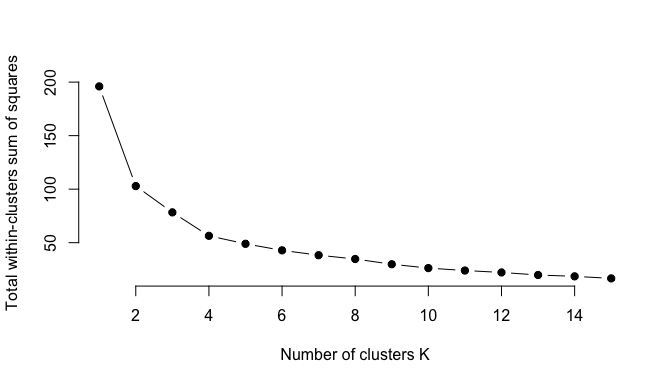
\includegraphics[width=0.2\textwidth]{lectures/slides_tex/figures/elbow_detection.png}
        \end{figure}
        \item Other methods: Gap analysis
    \end{itemize}
\end{frame}


\begin{frame}{Hierarchical Clustering}
    \begin{itemize}
        \item Does not require specific of number of clusters.
        \item Require dissimilarity measure.
        \item Produce hierarchical representations in which the clusters at each level of the hierarchy are created by merging clusters at the next lower level. 
        \item Two paradigms: agglomerative (bottom-up merging) and divisive (top-down splitting).
        \item Typically shown in a dendrogram.
    \end{itemize}
\end{frame}


\begin{frame}{Recent application: Lithium Superionic Conductors}
\begin{figure}
    \centering
    \includegraphics[width=0.8\textwidth]{figures/hirerachicalclustering-superionicconductors.pdf}
    \caption{a. Dendrogram generated using the agglomerative hierarchical clustering method. The dashed line shows the position where all compounds are partitioned into seven groups, marked as I–VII from left to right and distinguished by different colors. b Mapping the dendrogram to the conductivity reveals the grouping of known solid-state Li-ion conductors in group V and VI. Reproduced from \cite{zhangUnsupervisedDiscoverySolidstate2019}.}
\end{figure}
\end{frame}


\begin{frame}{Density-based Clustering}
    \begin{itemize}
        \item Clusters are defined as areas of higher density.
        \item Most popular variant is Density-based spatial clustering of applications with noise (DBSCAN).\cite{esterDensityBasedAlgorithmDiscovering}
        \item DBSCAN groups together points that are closely packed together and marks points that lie alone in low-density regions as outliers. 
        \item Key parameters of the DBSCAN algorithm are:
        \begin{itemize}
            \item eps: Max distance between two samples for one to be considered as in the neighborhood of the other. 
            \item min\_samples: No. of samples in a neighborhood for a point to be considered as a core point.
        \end{itemize}
    \end{itemize}
\end{frame}


\begin{frame}[fragile]{K-means and DBSCAN in scikit-learn}
\inputminted{python}{example_sklearn_clustering.py}
\end{frame}



\begin{frame}[allowframebreaks]{Bibliography}
    \bibliographystyle{unsrt}
    \bibliography{refs}
\end{frame}




\begin{frame}
    \Huge{\centerline{The End}}
\end{frame}

\end{document}

